\section{Layer Demand Is Heterogeneous}
\label{sec:heterogeneity}

\begin{figure}[t]
    \centering
    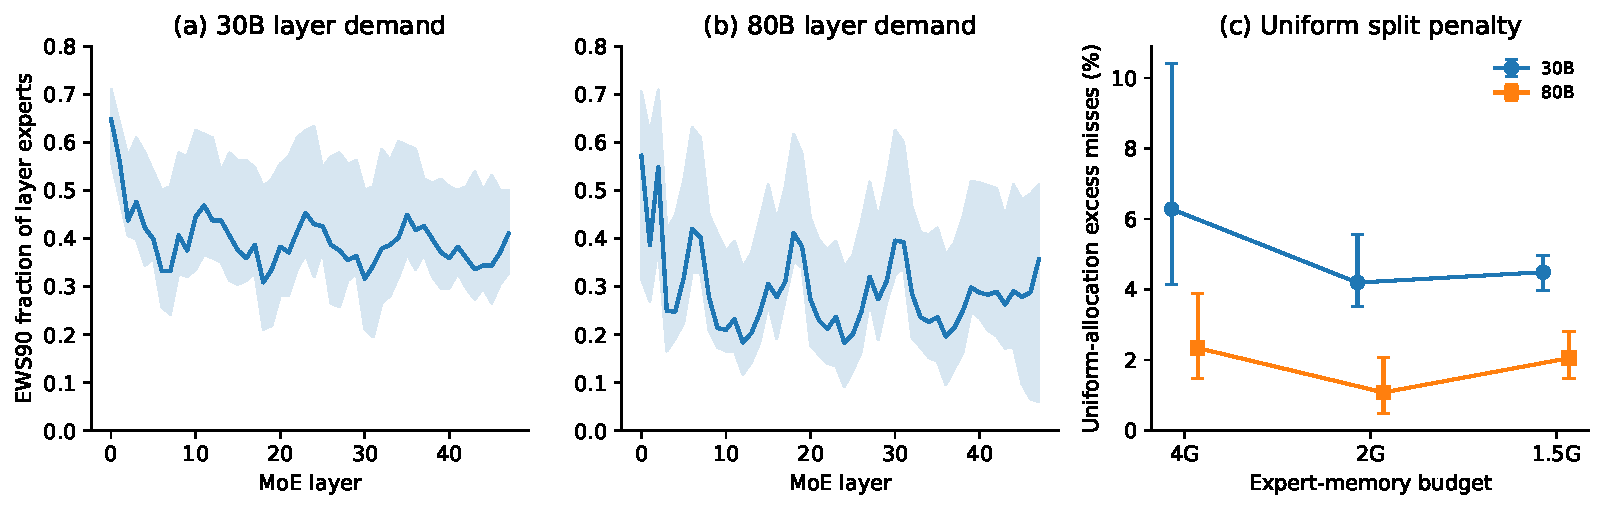
\includegraphics[width=\linewidth]{../experiments/EXP-007-router-characterization/figures/layer_heterogeneity_and_uniform_penalty.pdf}
    \caption{Layer demand is heterogeneous and uniform memory partitioning is measurably suboptimal. Panels (a) and (b) show the median per-layer EWS90 fraction across the 14 final in-sample workload/split cells for the 30B and 80B MoEs; shaded regions denote the full observed range. Layer-demand heterogeneity is present in both models, with per-cell EWS90 coefficients of variation spanning 0.085--0.248 for 30B and 0.162--0.455 for 80B. Panel (c) shows the median excess misses induced by a uniform per-layer memory split, with whiskers denoting the full observed range. The result establishes measurable allocation opportunity but does not imply that greater routing heterogeneity necessarily yields greater allocation benefit.}
    \label{fig:heterogeneity}
\end{figure}

The first question is whether a fixed expert-memory budget should be divided uniformly across MoE layers. If all layers exposed similar routed demand, a uniform partition would be a natural default. The EXP-007 characterization rejects that simplifying assumption within the evaluated traces.

Across the 14 final workload/split cells per model, global EWS90 fractions span approximately 0.327--0.554 for the 30B and 0.225--0.472 for the 80B. More importantly for allocation, the layer-by-layer working sets are not uniform within a trace. The coefficient of variation of per-layer EWS90 fractions ranges from 0.085 to 0.248 for the 30B and from 0.162 to 0.455 for the 80B. Figure~\ref{fig:heterogeneity}(a,b) shows that this heterogeneity is structured across depth rather than being a small perturbation around one common layer demand.

\subsection{The cost of a uniform layer split}

We quantify the allocation opportunity by replaying the same qualified routing trace under the same total memory budget while changing only the layer partition. Let $m_{\mathrm{uniform}}$ be the miss count obtained by splitting the budget uniformly across layers, and let $m_{\mathrm{static}}^{*}$ be the minimum miss count obtained by the in-sample static layer-allocation reference for that trace. We report the uniform-allocation excess
\begin{equation}
    E_{\mathrm{uniform}}
    =
    100\,
    \frac{m_{\mathrm{uniform}}-m_{\mathrm{static}}^{*}}
         {m_{\mathrm{static}}^{*}}
    \quad [\%].
    \label{eq:uniform-excess}
\end{equation}

The penalty is consistently larger for the 30B regime. Across the tested workload/split cells and budgets, the 30B uniform split incurs approximately 3.5--10.4\% excess misses, whereas the 80B incurs approximately 0.5--3.9\%. The effect is not explained by the 80B being more uniform. In fact, the 80B has the larger per-layer EWS spread, while exposing less exploitable inter-layer allocation opportunity.

The multi-turn workload makes this distinction concrete. Its 80B EWS90 fraction is lower than the 30B's, indicating more concentrated routing, yet its uniform-allocation penalty is substantially smaller. More generally, within each model there is an exploratory association between routing concentration and allocation opportunity, but that relationship does not transfer across models. Routing concentration is therefore not a model-agnostic proxy for the value of re-partitioning memory.

\begin{proposition}[Uniform layer allocation is suboptimal in the evaluated replay traces]
\label{prop:uniform-suboptimal}
For both evaluated MoE models, there exist qualified workload/split cells and memory budgets for which a non-uniform static allocation produces fewer misses than an equal per-layer split at the same global budget $M$.
\end{proposition}

\begin{proof}
EXP-007 replays identical qualified routing events at fixed $M$ while varying only the layer allocation. The measured excess in Eq.~\eqref{eq:uniform-excess} is strictly positive over the reported ranges, reaching 10.4\% for the 30B and 3.9\% for the 80B. Hence an equal split is not miss-minimal for those traces.
\end{proof}

The proposition is deliberately scoped. The comparator $m_{\mathrm{static}}^{*}$ is fitted to the same trace and therefore represents an in-sample memory-value reference, not an online policy and not an untouched out-of-sample result. The conclusion is that measurable layer-allocation opportunity exists; it does not establish that a particular adaptive controller can recover it in deployment.
